
\documentclass[]{article}

\title{La frecuencia de uso de palabras en el libro:
 Precepts in Practice; or, Stories Illustrating the Proverbs by A. L. O. E.}

\date{}
\usepackage{braket}
\usepackage{bbold}
\usepackage{amsmath,amsfonts,amssymb,amsthm}
\usepackage[margin=1.0in]{geometry}
\usepackage{graphicx}
\usepackage{chngcntr}
\usepackage{floatrow}
\usepackage{chngcntr}
\usepackage{hyperref}

\counterwithin{figure}{section}
\usepackage[backend=biber]{biblatex}
\addbibresource{ref.bib}
\begin{document}
	\maketitle
	\begin{center}


\centerline{\textbf{TAREA 2} } 
\textbf{ }

\centerline{Alumno: } 
\centerline{Joaquín Arturo Velarde Moreno}


	\end{center}
	

\section{Introducción:}

En el presente trabajo se hizo el análisis de la frecuencia en el uso de una selección de palabras y letras contenidas en el libro de Precepts in Practice; or, Stories Illustrating the Proverbs del autor A. L. O.  \cite{proverbs} 
Este libro se encuentra en la biblioteca digital de Gutenberg  \cite{guten},  el cual es el repositorio de más de 63,127 títulos en formato ebook.

Esta obra que revisamos está escrita en inglés y se conforma por un conjunto de relatos cuyas ilustraciones tienen el objetivo de complementar visualmente cada proverbio y, de acuerdo con este género literario, cada historia conlleva una enseñanza de la que podemos aprender en nuestra vida cotidiana, según las diferentes situaciones y asuntos de que se trate.

\section{Metodología:}
Para cumplir con nuestro objetivo, primeramente, procedimos a descargar el texto con el programa “R- 4.0.2” \cite{rproject}., dado que la biblioteca Gutenberg \cite{guten} permite tal descarga libremente.
Como siguiente paso, se removió todo carácter especial no alfa numérico, es decir, los símbolos tipográficos (guiones, cursivas, negritas, etc.) para limpiar el texto.
Debido a que la frecuencia de datos era dominada principalmente por artículos, pronombres personales, conjunciones y números, se hizo una hoja de datos en Microsoft Excel \cite{excel} con este tipo de palabras. Posteriormente, se le ordenó al programa limpiar el texto de dichos caracteres.
Con el resto del léxico, se pudo calcular la frecuencia de dichas palabras en dos áreas:


\begin{enumerate}
	\item Análisis de letras
	\item Análisis de palabras

\end{enumerate}


\subsection{Análisis de grafías:}
Para efectuar el análisis de grafías, se creó un diagrama de cajas y bigotes que representan la frecuencia de aparición de las letras enek el texto \autoref{fig:boxplot}, obteniendo los siguientes datos: mínimo, máximo, media, primer cuartil y tercer cuartil utilizando, como se señaló antes, el programa R 4.0.2  \cite{rproject}. 

\begin{figure}[b]
    \centering
    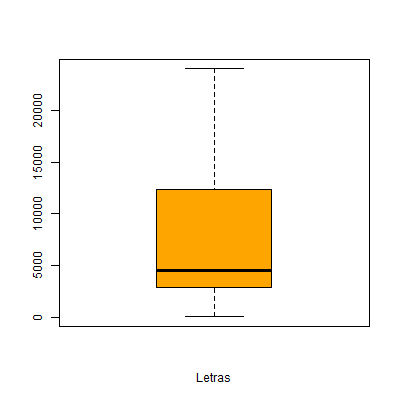
\includegraphics[width=.5\linewidth]{boxplot.png}    \caption{Frecuencia de letras representado en diagrama de cajas}
    \label{fig:boxplot}
\end{figure}

Se decidió, para mayor claridad, dar un enfoque al conjunto que inicia desde el segundo quantil y cuarto quantil obtenidas con la función \textit{summary()} para, de este modo, concentrar las frecuencias en un rango más cercano. 
 Con esta información se elaboró una figura de barras en la que se muestra la frecuencia de las letras, descubriendo un predominio de una serie de consonantes como son: s, r, d, l, u, w, m, f, c, g, y, p ordenadas de mayor a menor frecuencia, tal y como se muestra en el gráfico 
\autoref{fig:letras}
\begin{figure}[b]
    \centering
    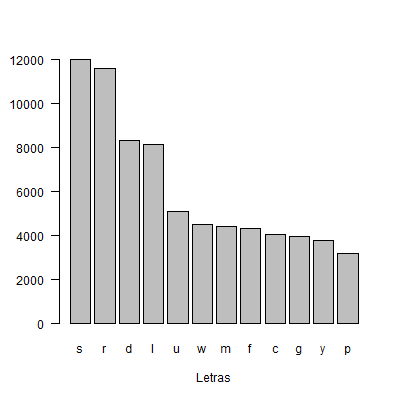
\includegraphics[width=.5\linewidth]{Letras.png}    \caption{Frecuencia de letras representado en diagrama}
    \label{fig:letras}
\end{figure}

\subsection{Análisis de palabras:}
Con la utilización del programa mencionado, también pudimos obtener información acerca de la frecuencia de las palabras y su cantidad contenidas del segundo quantil hasta el cuarto quantil del resumen dado por la function summary() para así concentrar el léxico más frecuente. 

\autoref{fig:palabras}
\begin{figure}[b]
    \centering
    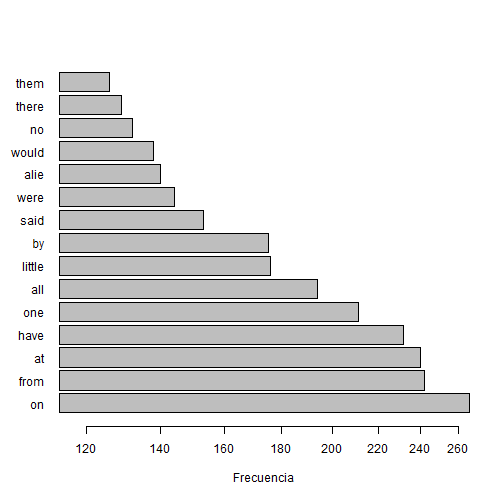
\includegraphics[width=.5\linewidth]{Palabras.png}    \caption{Frecuencia de Palabras representado en diagrama}
    \label{fig:palabras}
\end{figure}


\printbibliography[title={Referencias}]
\end{document}
